%----------------------------------------------------------------------------------------
%   CV - Jun-yu Jiang
%   Based on Jitin Nair template, modified for XeLaTeX with photo
%----------------------------------------------------------------------------------------
\documentclass[a4paper,12pt]{article}

%----------------------------------------------------------------------------------------
%   FONT
%----------------------------------------------------------------------------------------
\usepackage{fontspec}
\usepackage{xeCJK}
% Body: a refined serif. Prefer Playfair Display headings + EB Garamond body if available.
\IfFontExistsTF{EB Garamond}{%
  \setmainfont{EB Garamond}[Ligatures=TeX, Numbers=OldStyle]
}{%
  \setmainfont{Times New Roman}
}
\setsansfont{Helvetica Neue}
% CJK fallback so the single Chinese token "豆瓣" in the header renders cleanly.
\setCJKmainfont{Songti SC}
\setCJKsansfont{PingFang SC}
% Display font for the name — Playfair Display preferred, Garamond fallback.
\IfFontExistsTF{Playfair Display}{%
  \newfontfamily{\namefont}{Playfair Display}[LetterSpace=4.0]
}{%
  \IfFontExistsTF{Garamond}{%
    \newfontfamily{\namefont}{Garamond}[LetterSpace=4.0]
  }{%
    \newfontfamily{\namefont}{Times New Roman}[LetterSpace=4.0]
  }%
}

%----------------------------------------------------------------------------------------
%   PACKAGES
%----------------------------------------------------------------------------------------
\usepackage{url}
\usepackage{parskip}
\RequirePackage{color}
\RequirePackage{graphicx}
\usepackage[usenames,dvipsnames]{xcolor}
\usepackage[scale=0.9]{geometry}
\usepackage{tabularx}
\usepackage{enumitem}
\newcolumntype{C}{>{\centering\arraybackslash}X}
\usepackage{supertabular}
\usepackage{titlesec}
\usepackage{multicol}
\usepackage{multirow}
\usepackage{amssymb}
\usepackage{fontawesome5}

% Section formatting: small caps with rule (matching original)
\titleformat{\section}{\Large\scshape\raggedright}{}{0em}{}[\titlerule]
\titlespacing{\section}{0pt}{10pt}{10pt}

% Page background — light grey-white for a refined feel
\usepackage{xcolor}
\definecolor{pagebg}{HTML}{F7F7F5}
\usepackage{pagecolor}
\pagecolor{pagebg}

% Hyperlinks
\usepackage[unicode, draft=false]{hyperref}
\definecolor{linkcolour}{HTML}{2B6CB0}   % refined professional blue
\definecolor{doubangreen}{HTML}{2A8C3F}  % Douban-style green
\definecolor{fbblue}{HTML}{1877F2}       % official Facebook blue
\hypersetup{colorlinks,breaklinks,urlcolor=linkcolour,linkcolor=linkcolour}

%----------------------------------------------------------------------------------------
\begin{document}
\pagestyle{empty}

%----------------------------------------------------------------------------------------
%   HEADER: PHOTO + NAME/CONTACT
%----------------------------------------------------------------------------------------
\noindent
\begin{minipage}[c]{0.20\textwidth}
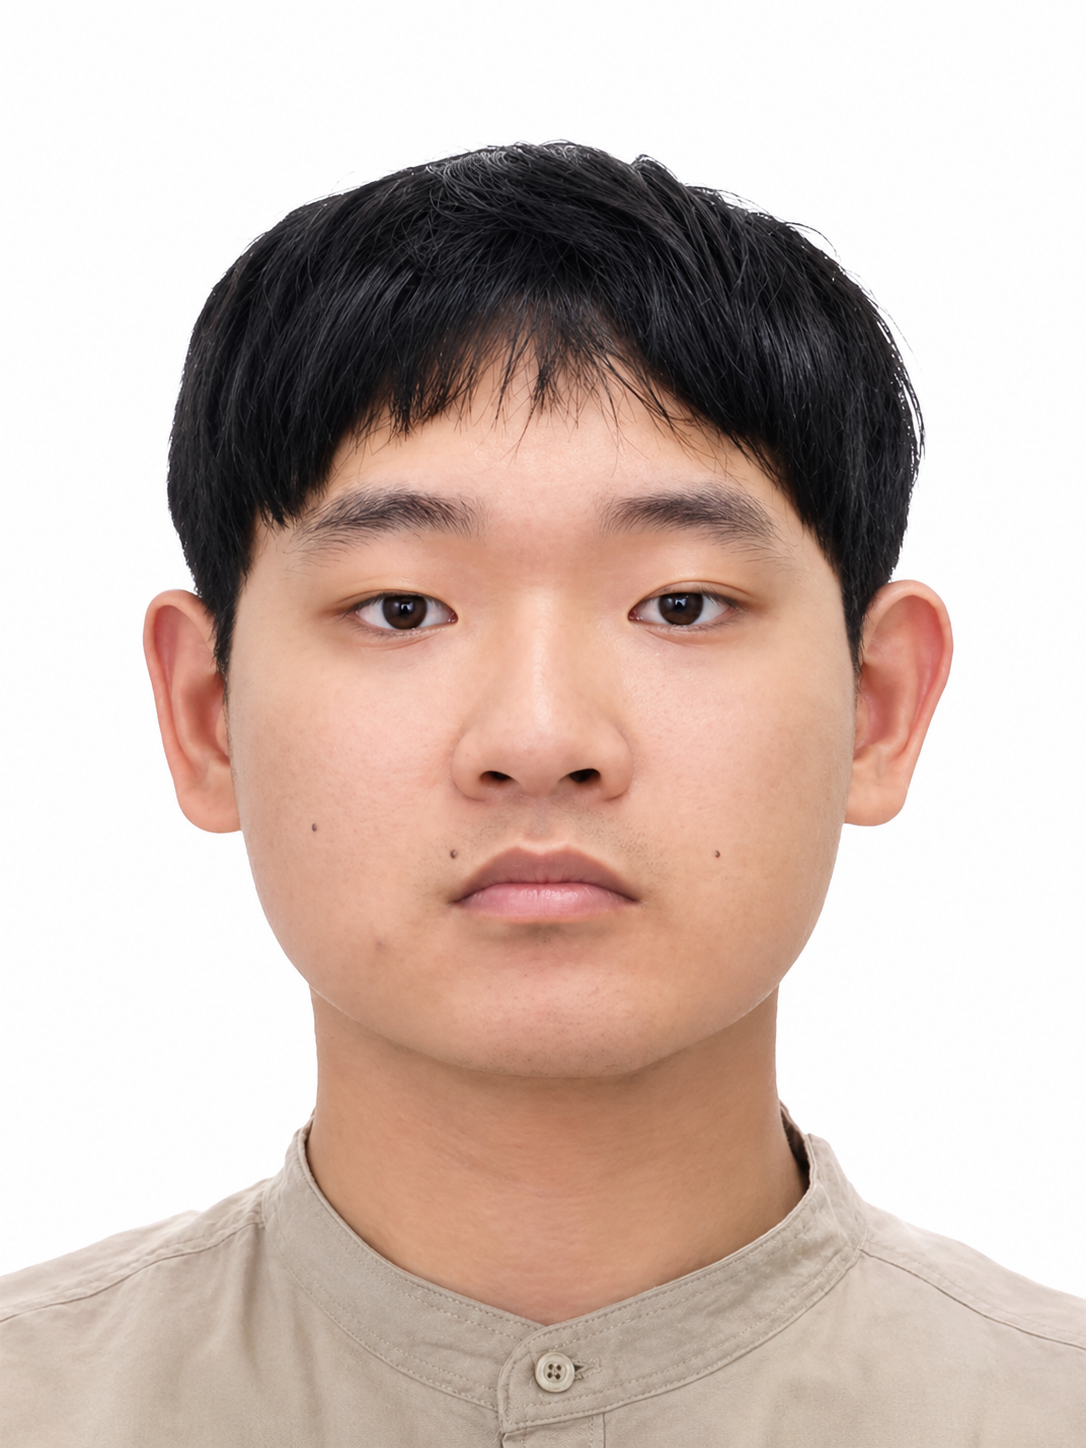
\includegraphics[width=\linewidth]{photo-for-cv.png}
\end{minipage}%
\hfill
\begin{minipage}[c]{0.78\textwidth}
\begin{center}
\vspace{50pt}
% Name — large refined serif with subtle letter-spacing
{\namefont\fontsize{40}{44}\selectfont Li Zihao}\\[14pt]
% Top row: 3 primary contacts
{\sffamily\small\color{linkcolour}%
  \href{https://chiselli.com}{\faGlobe\,\,chiselli.com}\hspace{2.2em}%
  \href{mailto:lizihao2023@lzu.edu.cn}{\faEnvelope[regular]\,\,lizihao2023@lzu.edu.cn}\hspace{2.2em}%
  \href{https://github.com/MiShenng}{\faGithub\,\,MiShenng}%
}\\[8pt]
% Bottom row: 2 secondary social contacts, centered beneath
{\sffamily\small%
  \href{https://www.douban.com/people/MiShenng}{\color{doubangreen}\faBookOpen}\,\,{\color{linkcolour}\href{https://www.douban.com/people/MiShenng}{Douban}}\hspace{2.6em}%
  \href{https://www.facebook.com/chiselli}{\color{fbblue}\faFacebookF}\,\,{\color{linkcolour}\href{https://www.facebook.com/chiselli}{Facebook}}%
}
\end{center}
\end{minipage}

\vspace{6pt}

%----------------------------------------------------------------------------------------
%   EDUCATION
%----------------------------------------------------------------------------------------
\section{Education}

\begin{tabularx}{\linewidth}{@{}X r@{}}
$\bullet$ \textbf{Lanzhou University, Lanzhou} & \textit{Sep. 2023 -} \\
\end{tabularx}
\quad \textit{B.A. in Journalism}\\
\quad\quad $\circ$ \textbf{Relevant Coursework:} New Media User Analysis, Communication Psychology, Media Criticism, Research Methods in Communication Studies, Data Journalism, Introduction to Communication Studies, Public Opinion\\
\quad\quad $\circ$ \textbf{GPA: \href{https://mybolg-lizao.vercel.app/media/pdfs/lanzhou_transcript_en.pdf}{4.05/5.0}}

\vspace{4pt}

\begin{tabularx}{\linewidth}{@{}X r@{}}
$\bullet$ \textbf{National Taiwan Normal University, Taipei} & \textit{Aug. 2025 - Dec. 2025} \\
\end{tabularx}
\quad \textit{Exchange Student}\\
\quad\quad $\circ$ \textbf{Relevant Coursework:} Visual Culture and Communication, Research Method of Social Science, New Media and Society Seminar\\
\quad\quad $\circ$ \textbf{GPA: \href{https://mybolg-lizao.vercel.app/media/pdfs/taiwan_transcript.pdf}{3.9/4.0}}



%----------------------------------------------------------------------------------------
%   PUBLICATIONS
%----------------------------------------------------------------------------------------
\section{Peer-reviewed publications \& Conference Papers}

\begin{tabularx}{\linewidth}{@{}X r@{}}
\textbf{$\bullet$ Should I Stay Calm: How Does the Combination of Visual and Textual Frames Influence Expressions of Anger in Short Video Comment Sections?} & \textit{AEJMC 2026} \\
\end{tabularx}
\quad \textit{Li, Zihao.*} \hfill [\href{https://some-link.com}{\faGlobe}]
\begin{itemize}[nosep, leftmargin=2em, itemsep=3pt, label=$\circ$]
\item This study develops a computational method for identifying visual frames in dynamic short videos, applied to 449 Douyin videos on China's drug record sealing controversy alongside 419,126 user comments. Both visual and textual content are classified into intensifying, informational, and mitigating frames, while a fine-tuned BERT classifier ($F_1 = 0.972$) detects anger at the comment level.
\item Results show that visual and textual frames within individual videos tend to align rather than diverge, and that different frame combinations correspond to significantly different levels of comment anger. Two-way ANOVA confirms that both modalities independently contribute to anger in an additive fashion without significant interaction, suggesting that emotional responses are jointly organized across modalities rather than driven by a single channel.
\end{itemize}

\vspace{6pt}

\begin{tabularx}{\linewidth}{@{}X r@{}}
\textbf{$\bullet$ Negotiating the Future of Artificial Intelligence in Everyday Talk: Sociotechnical Imaginaries of Chinese Coding Elites in Podcasts} & \textit{NCA 2026} \\
\end{tabularx}
\quad \textit{Li, Zihao.*} \hfill [\href{https://some-link.com}{\faGlobe}]
\begin{itemize}[nosep, leftmargin=2em, itemsep=3pt, label=$\circ$]
\item This study examines how Chinese coding elites construct sociotechnical imaginaries of AI through podcast conversations, drawing on 432 episodes from Xiaoyuzhou analyzed via BERTopic modeling and discourse analysis. Rather than passively reproducing state or corporate narratives, coding elites produce a cautious yet legitimizing vision of AI futures within this semi-public communicative space.
\item Their discourse navigates tensions among global technology centers, national strategic aspirations, and local application realities, sustaining a spectrum of AI identities from instrumental tool to quasi-social partner. Three rhetorical resources underpin these imaginaries: technological feasibility, market liberalism, and national development narratives.
\end{itemize}

\vspace{6pt}

%----------------------------------------------------------------------------------------
%   WORKING PAPERS
%----------------------------------------------------------------------------------------
\section{Working Papers \& Research in Progress}

\begin{tabularx}{\linewidth}{@{}X r@{}}
\textbf{$\bullet$ See It, Click It? How Visual Clickbait Shapes Stratified User Engagement in Health-Related Videos on China's Bilibili} & \textit{ICSC 2026} \\
\end{tabularx}
\quad \textit{Li, Zihao.*} \hfill \textit{Research in Progress} \quad [\href{https://some-link.com}{\faGlobe}]
\begin{itemize}[nosep, leftmargin=2em, itemsep=3pt, label=$\circ$]
\item This study investigates how visual clickbait cues in health video thumbnails shape stratified user engagement on Bilibili, drawing on 22,323 health-related video entries. Visual clickbait is operationalized along four dimensions (emotional valence, health threat symbols, visual pressure, and information gaps) through a human-machine hybrid annotation workflow.
\item A cost-stratified engagement framework distinguishes low-cost attention such as views and likes from high-cost endorsement such as coin donation, testing whether thumbnails that attract clicks also earn deeper user commitment. Semantic congruence between thumbnails and titles, quantified via Chinese-CLIP cosine similarity, is introduced as a moderating variable in the regression analysis.
\end{itemize}

%----------------------------------------------------------------------------------------
%   RESEARCH EXPERIENCE
%----------------------------------------------------------------------------------------
\section{Research Experience}

\begin{tabularx}{\linewidth}{@{}X r@{}}
\textbf{$\bullet$ A Study on Discourse Construction and Visual Narrative Strategies in the New Mainstream Media Environment of the Converged Media Era} & \textit{Dec. 2024 - Apr. 2025} \\
\end{tabularx}
\textit{PI: Li xinxin, Lanzhou  University} \quad [\href{https://some-link.com}{\faGlobe}] \hfill \textbf{Rearch Assistant}
\begin{itemize}[nosep, leftmargin=2em, itemsep=3pt, label=$\circ$]
\item Basic Research Projects of Central Universities in China
\item Using reports from the People’s Daily as representative examples of mainstream media, I constructed a dataset of environmental news coverage from 1949 to the present. I then developed an LLM-driven automated content analysis program to perform coding. Applying Fairclough’s discourse analysis methodology and combining the coding results with the evolution of China’s environmental protection policies, I broadly divided the historical development of China’s environmental protection discourse into distinct phases.
\item Using a self-built web crawler to collect Weibo posts related to environmental protection from the People's Daily to date, and conducted a comparative analysis of this data with content from the newspaper's print editions.
\end{itemize}

\vspace{6pt}

\begin{tabularx}{\linewidth}{@{}X r@{}}
\textbf{$\bullet$ A Study on the “Human-Machine Co-creation” Mechanism and Innovative Practices in AI-Empowered Cultural Narratives Along the Silk Road} & \textit{Mar. 2025 - May. 2025} \\
\end{tabularx}
\textit{PI: Li xinxin, Lanzhou  University} \quad [\href{https://some-link.com}{\faGlobe}] \hfill \textbf{Research Assistant}
\begin{itemize}[nosep, leftmargin=2em, itemsep=3pt, label=$\circ$]
\item Compilation of narrative resources on the history of the Silk Road
\item Compile the research trends in various social sciences related to the Silk Road and write a comprehensive review
\end{itemize}

\vspace{6pt}

\begin{tabularx}{\linewidth}{@{}X r@{}}
\textbf{$\bullet$ Lanzhou Bathing Assistant：Seeing Aging at Mobile Bathhouses} & \textit{Aug. 2024 - Jan. 2025} \\
\end{tabularx}
\textit{Advisor: Shiping, Lanzhou University} \quad [\href{https://some-link.com}{\faGlobe}]  \hfill \textbf{Field Research}
\begin{itemize}[nosep, leftmargin=2em, itemsep=3pt, label=$\circ$]
\item Conducted ethnographic field research on the emerging in-home elder-bathing industry in Lanzhou, examining how disabled and bedridden older adults navigate bodily dignity, agency, and social invisibility under China's home-based eldercare model. Performed on-site participant observation of bathing services and semi-structured interviews with the company founder, bathing assistants, eldercare-center managers, and family caregivers.
\item Situated individual narratives within China's accelerating demographic transition, analyzing structural barriers --- arid climate, limited water infrastructure, and deeply rooted cultural attitudes toward death and the aging body --- that impede the industry's expansion in northwest China. This resulted in an in-depth written report and a short video documentary.
\end{itemize}

\vspace{6pt}

\begin{tabularx}{\linewidth}{@{}X r@{}}
\textbf{$\bullet$ Why Do College Students Have a Particular Affinity for Life “Within the System”?
—A Mechanism Analysis of College Students’ Employment Behavior and Policy Recommendations
} & \textit{Apr. 2024 - Apr. 2025} \\
\end{tabularx}
\textit{Advisor: Zhangchi, Lanzhou University} \quad [\href{https://mybolg-lizao.vercel.app/media/pdfs/lanzhou_transcript.pdf}{\faGlobe}] \hfill \textbf{Co Worker}
\begin{itemize}[nosep, leftmargin=2em, itemsep=3pt, label=$\circ$]
\item Investigated the behavioral mechanisms driving Chinese college students' intensifying preference for public-sector employment. Co-designed the survey instrument, oversaw questionnaire distribution and data collection, and performed statistical analysis to isolate key predictors of career-choice behavior.
\item Complemented quantitative findings with semi-structured interviews, triangulating survey data with personal narratives to unpack the motivations fueling the civil-service-exam craze (\textit{kaogong} fever) and to formulate evidence-based policy recommendations.
\end{itemize}

\vspace{6pt}

%----------------------------------------------------------------------------------------
%   AWARDS
%----------------------------------------------------------------------------------------
\section{Selected Awards and Honors}

% Each award uses two rows: title (bold) on row 1, level (italic, gray) + date on row 2
\newcommand{\awarditem}[3]{%
$\bullet$ \textbf{#1} \\
\quad \textit{\textcolor{gray}{#2}} \hfill \textit{#3} \\[4pt]
}

\noindent
\awarditem{China Data Journalism Competition}{Second Prize (National Level)}{Nov. 2025}
\awarditem{China Statistical Modeling Competition}{First Prize (Provincial Level)}{May. 2026}
\awarditem{Central China Mathematical Modeling Competition}{Second Prize (Provincial Level)}{May. 2026}
\awarditem{China University Campus Media Competition}{Public Service Communication Award(Provinvial Level)}{Nov. 2025}
\awarditem{14th China Tower Journalists' Day}{Grand Prize in the Communications Category(Provincial Level)}{Dec. 2025}
\awarditem{Lanzhou University Outstanding Student Scholarship}{University Level}{Sep. 2023 - Sep. 2024}

%----------------------------------------------------------------------------------------
%   SKILLS
%----------------------------------------------------------------------------------------
\section{Skills}

\begin{tabularx}{\linewidth}{@{}l X@{}}
\textbf{Programming} &  Python, R, Web (HTML, CSS, JavaScript), AI4SS \\
\textbf{Analytical Tools} &  SPSS, NVivo \\
\textbf{NLP/ML Models} &  BERT, LDA, and other transformer-based architectures \\
\textbf{Production Tools} &  \LaTeX, Microsoft Office Suite, Photography \\
\textbf{Language} &  IELTS(6.5), Cet6(530), Cet4(518), Mandarin \\
\end{tabularx}



\end{document}




%----------------------------------------------------------------------------------------
%   WORK EXPERIENCE
%----------------------------------------------------------------------------------------
\section{Selected Work Experience}

\begin{tabularx}{\linewidth}{@{}X r@{}}
\textbf{$\bullet$ China Telecom} & \textit{Jan. 2022 - Mar. 2022} \\
\end{tabularx}
\textit{Event Operations Intern}
\begin{itemize}[nosep, leftmargin=2em, itemsep=3pt, label=$\circ$]
\item Analyzed real-time social media data (Weibo, WeChat) to model user engagement patterns and public opinion trends.
\item Performed large-scale comment analysis to identify key audience demographics and public sentiment, guiding content development.
\end{itemize}

\vspace{6pt}

\begin{tabularx}{\linewidth}{@{}X r@{}}
\textbf{$\bullet$ iFeng} & \textit{Sep. 2023 - Dec. 2023} \\
\end{tabularx}
\textit{News Editing Intern} \hfill [\href{https://some-link.com}{\faGlobe}]
\begin{itemize}[nosep, leftmargin=2em, itemsep=3pt, label=$\circ$]
\item Authored and published press releases on emerging technology for iFeng.com, covering major industry events.
\item Developed video scripts for the \textit{ifengTech} column and conducted daily public opinion monitoring, providing analytical briefings.
\end{itemize}
